
\section{Abbildungen/Funktionen}

\textbf{Definition (Abbildung oder Funktion):}

Seien $A$ und $B$ zwei Mengen. Eine Abbildung
$f:A\rightarrow B$ ordnet jedem $x\in A$ genau
ein Element $f(x)\in B$ zu:
\[
f:A\rightarrow B,\qquad x\mapsto f(x).
\]
$A$ heißt Definitionsbereich und $B$ Zielmenge.
Das tatsächliche Bild ist eine Teilmenge der Zielmenge.
Für $A\subseteq\mathbb R$ und $B\subseteq\mathbb R$
liegt insbesondere eine reellwertige Funktion
einer reellen Variablen vor.

Beispiel:\\
\textbullet $\qquad f_1:\mathbb{R}\rightarrow \mathbb{R}\text{ ,  }  x\rightarrow 2x $\vspace*{2mm}\\
\begin{center}
	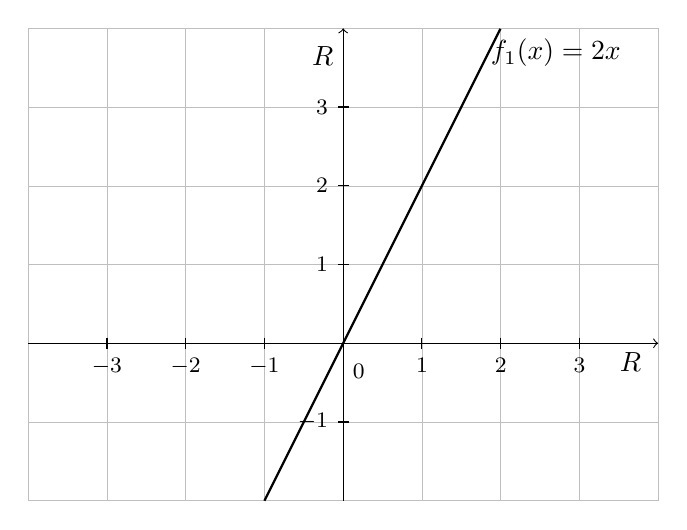
\begin{tikzpicture}
		
		% Gitternetzlinien
		\draw[xstep=1cm, ystep=1cm, very thin, color=lightgray] (-4,4) grid (4,-2);
		% x-Achse
		\draw[->] (-4,0) -- (4,0) node[below,xshift=-1em] {$\mathbb{R}$}; 
		%Zahlen auf x-Achse
		\foreach \x in {-3,...,-1}
		\draw[shift={(\x,0)},color=black] (0pt,2pt) -- (0pt,-2pt) node[below] {\footnotesize $\x$};
		\foreach \x in {1,...,3}
		\draw[shift={(\x,0)},color=black] (0pt,2pt) -- (0pt,-2pt) node[below] {\footnotesize $\x$};
		% y-Achse 
		\draw[->] (0,-2) -- (0,4) node[left,yshift=-1em] {$\mathbb{R}$};%node[above left]
		%Zahlen auf y-Achse
		\foreach \y in {-1,...,-1}
		\draw[shift={(0,\y)},color=black] (2pt,0pt) -- (-2pt,0pt) node[left] {\footnotesize $\y$};
		\foreach \y in {1,...,3}
		\draw[shift={(0,\y)},color=black] (2pt,0pt) -- (-2pt,0pt) node[left] {\footnotesize $\y$};
		%Ursprung
		\draw[color=black] (0pt,-10pt) node[right] {\footnotesize $0$};
		
		
		
		\draw[thick,color=black] plot[samples=200, domain=-1:2] 
		(\x,{2*\x}) node[below, xshift=2em]{$f_1(x)=2x$};
		
		
		
	\end{tikzpicture}\vspace*{8mm}\\
\end{center}
\textbullet $\qquad f_2:\mathbb{R}\rightarrow \mathbb{R}\text{ ,  }  x\rightarrow x^2 $\vspace*{2mm}\\
\begin{center}
	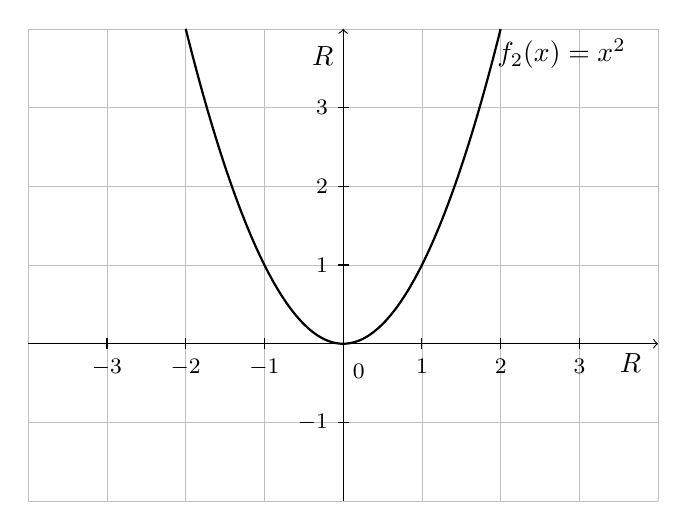
\begin{tikzpicture}
		
		% Gitternetzlinien
		\draw[xstep=1cm, ystep=1cm, very thin, color=lightgray] (-4,4) grid (4,-2);
		% x-Achse
		\draw[->] (-4,0) -- (4,0) node[below,xshift=-1em] {$\mathbb{R}$}; 
		%Zahlen auf x-Achse
		\foreach \x in {-3,...,-1}
		\draw[shift={(\x,0)},color=black] (0pt,2pt) -- (0pt,-2pt) node[below] {\footnotesize $\x$};
		\foreach \x in {1,...,3}
		\draw[shift={(\x,0)},color=black] (0pt,2pt) -- (0pt,-2pt) node[below] {\footnotesize $\x$};
		% y-Achse 
		\draw[->] (0,-2) -- (0,4) node[left,yshift=-1em] {$\mathbb{R}$};%node[above left]
		%Zahlen auf y-Achse
		\foreach \y in {-1,...,-1}
		\draw[shift={(0,\y)},color=black] (2pt,0pt) -- (-2pt,0pt) node[left] {\footnotesize $\y$};
		\foreach \y in {1,...,3}
		\draw[shift={(0,\y)},color=black] (2pt,0pt) -- (-2pt,0pt) node[left] {\footnotesize $\y$};
		%Ursprung
		\draw[color=black] (0pt,-10pt) node[right] {\footnotesize $0$};
		
		
		
		\draw[thick,color=black] plot[samples=200, domain=-2:2] 
		(\x,{\x*\x}) node[below, xshift=2.2em]{$f_2(x)=x^2$};
		
		
		
	\end{tikzpicture}\\
\end{center}
\newpage
\noindent
\textbullet  \;\;  Dies ist keine Abbildung.\\
\begin{center}
	
	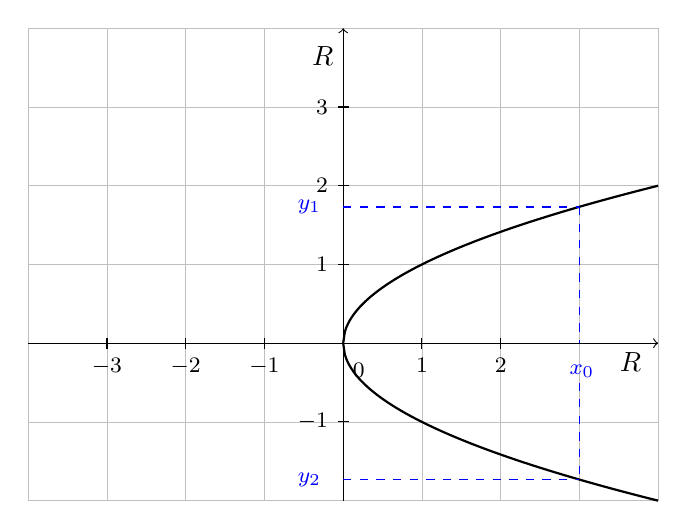
\begin{tikzpicture}
		
		% Gitternetzlinien
		\draw[xstep=1cm, ystep=1cm, very thin, color=lightgray] (-4,4) grid (4,-2);
		% x-Achse
		\draw[->] (-4,0) -- (4,0) node[below,xshift=-1em] {$\mathbb{R}$}; 
		%Zahlen auf x-Achse
		\foreach \x in {-3,...,-1}
		\draw[shift={(\x,0)},color=black] (0pt,2pt) -- (0pt,-2pt) node[below] {\footnotesize $\x$};
		\foreach \x in {1,...,2}
		\draw[shift={(\x,0)},color=black] (0pt,2pt) -- (0pt,-2pt) node[below] {\footnotesize $\x$};
		% y-Achse 
		\draw[->] (0,-2) -- (0,4) node[left,yshift=-1em] {$\mathbb{R}$};%node[above left]
		%Zahlen auf y-Achse
		\foreach \y in {-1,...,-1}
		\draw[shift={(0,\y)},color=black] (2pt,0pt) -- (-2pt,0pt) node[left] {\footnotesize $\y$};
		\foreach \y in {1,...,3}
		\draw[shift={(0,\y)},color=black] (2pt,0pt) -- (-2pt,0pt) node[left] {\footnotesize $\y$};
		%Ursprung
		\draw[color=black] (0pt,-10pt) node[right] {\footnotesize $0$};
		
		
		
		\draw[thick,color=black] plot[samples=200, domain=0:4] 
		(\x,{sqrt(\x)});
		
		\draw[thick,color=black] plot[samples=200, domain=0:4] 
		(\x,{-sqrt(\x)});
		\draw[color=blue] (-0.7,-1.73) node[right] {\footnotesize $y_2$};
		\draw[color=blue] (-0.7,1.73) node[right] {\footnotesize $y_1$};
		\draw[color=blue,dashed] (3,1.73) -- (3,0);
		\draw[color=blue,dashed] (3,-0.5) -- (3,-1.73);
		\draw[color=blue,dashed] (0,1.73) -- (3,1.73) ;
		\draw[color=blue,dashed] (0,-1.73) -- (3,-1.73);
		\draw[color=blue] (2.75,-10pt) node[right] {\footnotesize $x_0$};
	\end{tikzpicture}\\
\end{center}
Dies ist ein Widerspruch zur Definition einer Abbildung. Den Wert $x_0$ werden zwei Elemente und zwar $y_1$ und $y_2$ zugewiesen.\\
\subsection{Einschränkungen von Abbildungen}

\textbf{Definition (Einschränkung):}

Sei $f:D_f\rightarrow W_f$ eine Abbildung und
$C\subseteq D_f$. Die Einschränkung von $f$ auf $C$
ist die Abbildung
\[
f|_C:C\rightarrow W_f,\qquad
f|_C(x)=f(x)\quad\text{für alle }x\in C.
\]
Die Funktionsvorschrift bleibt gleich, nur der
Definitionsbereich wird eingeschränkt.

Beispiele:\\
\textbullet$\qquad f_2:\mathbb{R}\longmapsto [0,\infty[$ mit $x\longmapsto x^2$\\
\begin{center}
	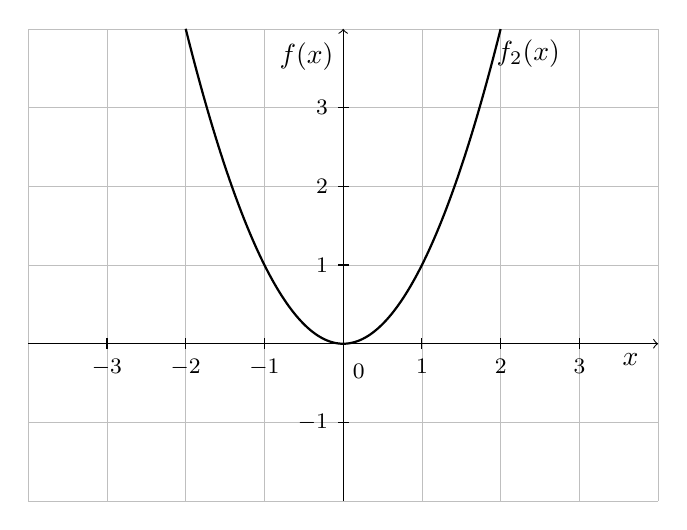
\begin{tikzpicture}
		
		% Gitternetzlinien
		\draw[xstep=1cm, ystep=1cm, very thin, color=lightgray] (-4,4) grid (4,-2);
		% x-Achse
		\draw[->] (-4,0) -- (4,0) node[below,xshift=-1em] {$x$}; 
		%Zahlen auf x-Achse
		\foreach \x in {-3,...,-1}
		\draw[shift={(\x,0)},color=black] (0pt,2pt) -- (0pt,-2pt) node[below] {\footnotesize $\x$};
		\foreach \x in {1,...,3}
		\draw[shift={(\x,0)},color=black] (0pt,2pt) -- (0pt,-2pt) node[below] {\footnotesize $\x$};
		% y-Achse 
		\draw[->] (0,-2) -- (0,4) node[left,yshift=-1em] {$f(x)$};%node[above left]
		%Zahlen auf y-Achse
		\foreach \y in {-1,...,-1}
		\draw[shift={(0,\y)},color=black] (2pt,0pt) -- (-2pt,0pt) node[left] {\footnotesize $\y$};
		\foreach \y in {1,...,3}
		\draw[shift={(0,\y)},color=black] (2pt,0pt) -- (-2pt,0pt) node[left] {\footnotesize $\y$};
		%Ursprung
		\draw[color=black] (0pt,-10pt) node[right] {\footnotesize $0$};
		
		
		
		\draw[thick,color=black] plot[samples=200, domain=-2:2] 
		(\x,{\x*\x}) node[below, xshift=1em]{$f_2(x)$};
		
		
		
	\end{tikzpicture}\\
\end{center}
\pagebreak
\textbullet $\qquad f_2|_{[0,\infty[}:[0,\infty[\; \longmapsto [0,\infty [\;$ mit $ x \longmapsto x^2 $\\
\begin{center}
	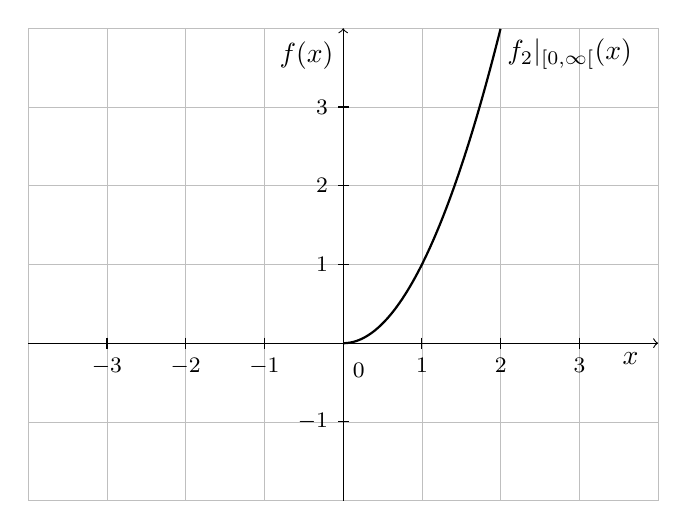
\begin{tikzpicture}
		% Gitternetzlinien
		\draw[xstep=1cm, ystep=1cm, very thin, color=lightgray] (-4,4) grid (4,-2);
		% x-Achse
		\draw[->] (-4,0) -- (4,0) node[below,xshift=-1em] {$x$}; 
		%Zahlen auf x-Achse
		\foreach \x in {-3,...,-1}
		\draw[shift={(\x,0)},color=black] (0pt,2pt) -- (0pt,-2pt) node[below] {\footnotesize $\x$};
		\foreach \x in {1,...,3}
		\draw[shift={(\x,0)},color=black] (0pt,2pt) -- (0pt,-2pt) node[below] {\footnotesize $\x$};
		% y-Achse 
		\draw[->] (0,-2) -- (0,4) node[left,yshift=-1em] {$f(x)$};%node[above left]
		%Zahlen auf y-Achse
		\foreach \y in {-1,...,-1}
		\draw[shift={(0,\y)},color=black] (2pt,0pt) -- (-2pt,0pt) node[left] {\footnotesize $\y$};
		\foreach \y in {1,...,3}
		\draw[shift={(0,\y)},color=black] (2pt,0pt) -- (-2pt,0pt) node[left] {\footnotesize $\y$};
		%Ursprung
		\draw[color=black] (0pt,-10pt) node[right] {\footnotesize $0$};
		\draw[thick,color=black] plot[samples=200, domain=0:2] 
		(\x,{\x*\x}) node[below, xshift=2.5em]{$f_2|_{[0,\infty[}(x)$};
		
		
		
	\end{tikzpicture}\\
\end{center}
Dies ist eine Funktion mit der Einschränkung von $f_2$ auf die Menge:$[0,\infty[$\vspace*{2mm}\\
\textbullet $\qquad f_1:\mathbb{R}\longmapsto\mathbb{R}\;$ mit $x\longmapsto 2x $\\

\begin{center}
	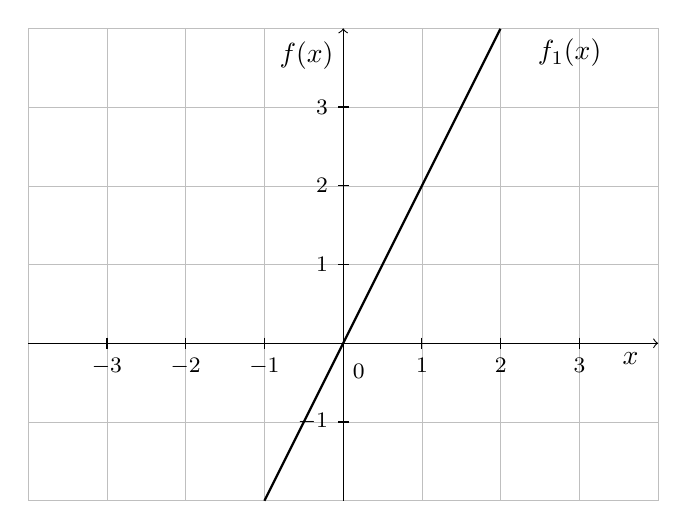
\begin{tikzpicture}
		% Gitternetzlinien
		\draw[xstep=1cm, ystep=1cm, very thin, color=lightgray] (-4,4) grid (4,-2);
		% x-Achse
		\draw[->] (-4,0) -- (4,0) node[below,xshift=-1em] {$x$}; 
		%Zahlen auf x-Achse
		\foreach \x in {-3,...,-1}
		\draw[shift={(\x,0)},color=black] (0pt,2pt) -- (0pt,-2pt) node[below] {\footnotesize $\x$};
		\foreach \x in {1,...,3}
		\draw[shift={(\x,0)},color=black] (0pt,2pt) -- (0pt,-2pt) node[below] {\footnotesize $\x$};
		% y-Achse 
		\draw[->] (0,-2) -- (0,4) node[left,yshift=-1em] {$f(x)$};%node[above left]
		%Zahlen auf y-Achse
		\foreach \y in {-1,...,-1}
		\draw[shift={(0,\y)},color=black] (2pt,0pt) -- (-2pt,0pt) node[left] {\footnotesize $\y$};
		\foreach \y in {1,...,3}
		\draw[shift={(0,\y)},color=black] (2pt,0pt) -- (-2pt,0pt) node[left] {\footnotesize $\y$};
		%Ursprung
		\draw[color=black] (0pt,-10pt) node[right] {\footnotesize $0$};
		\draw[thick,color=black] plot[samples=200, domain=-1:2] 
		(\x,{\x*2}) node[below, xshift=2.5em]{$f_1(x)$};
		
		
		
	\end{tikzpicture}\\
\end{center}
\textbullet $\qquad f_1|_{\mathbb{Z}}:\mathbb{Z}\longmapsto\mathbb{Z}\;$ mit $x\longmapsto 2x $$\qquad$ Bemerkung: ($\longmapsto\mathbb{Z}$, weil $2\cdot x$ immer $\in\mathbb{Z}$ ist)\\

\begin{center}
	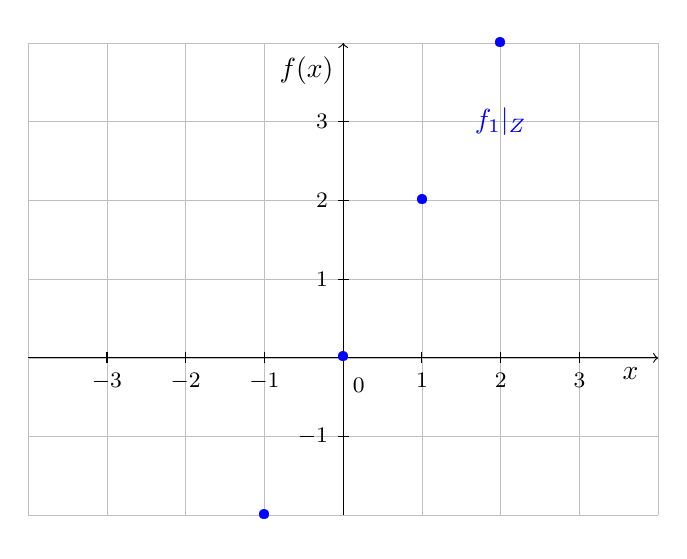
\begin{tikzpicture}
		% Gitternetzlinien
		\draw[xstep=1cm, ystep=1cm, very thin, color=lightgray] (-4,4) grid (4,-2);
		% x-Achse
		\draw[->] (-4,0) -- (4,0) node[below,xshift=-1em] {$x$}; 
		%Zahlen auf x-Achse
		\foreach \x in {-3,...,-1}
		\draw[shift={(\x,0)},color=black] (0pt,2pt) -- (0pt,-2pt) node[below] {\footnotesize $\x$};
		\foreach \x in {1,...,3}
		\draw[shift={(\x,0)},color=black] (0pt,2pt) -- (0pt,-2pt) node[below] {\footnotesize $\x$};
		% y-Achse 
		\draw[->] (0,-2) -- (0,4) node[left,yshift=-1em] {$f(x)$};%node[above left]
		%Zahlen auf y-Achse
		\foreach \y in {-1,...,-1}
		\draw[shift={(0,\y)},color=black] (2pt,0pt) -- (-2pt,0pt) node[left] {\footnotesize $\y$};
		\foreach \y in {1,...,3}
		\draw[shift={(0,\y)},color=black] (2pt,0pt) -- (-2pt,0pt) node[left] {\footnotesize $\y$};
		%Ursprung
		\draw[color=black] (0pt,-10pt) node[right] {\footnotesize $0$};
		
		
		\draw[color=blue] (1,2) node {\textbullet};
		\draw[color=blue] (2,4) node {\textbullet};
		\draw[color=blue] (0,0) node {\textbullet};
		\draw[color=blue] (-1,-2) node {\textbullet};
		\draw[color=blue] (2,3) node {$f_1|_{\mathbb{Z}}$};
		
	\end{tikzpicture}\\
\end{center}
\pagebreak
\subsection{Bild einer Abbildung}

\textbf{Definition (Bild):}\\
Sei $f:\mathbb{D}_f\longmapsto\mathbb{W}_f$ eine Abbildung.\\
Das Bild von $f$ ist die Menge:\\
\begin{align*}
	\mathrm{Bild}(f)=f(\mathbb{D}_f)=\{f(x)\mid x\in\mathbb{D}_f\}\subseteq\mathbb{W}_f
\end{align*}
Beispiele:\\
\textbullet$\qquad f_2:\mathbb{R}\longmapsto [0,\infty[ \qquad$ mit $x\longmapsto x^2$\\
\begin{center}
	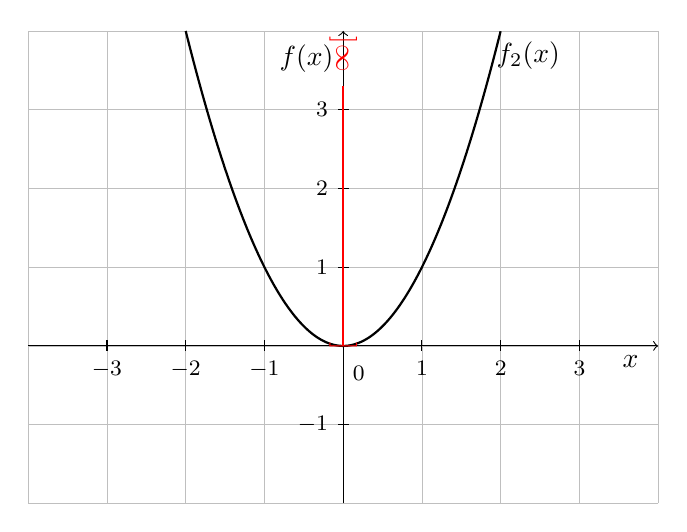
\begin{tikzpicture}
		
		% Gitternetzlinien
		\draw[xstep=1cm, ystep=1cm, very thin, color=lightgray] (-4,4) grid (4,-2);
		% x-Achse
		\draw[->] (-4,0) -- (4,0) node[below,xshift=-1em] {$x$}; 
		%Zahlen auf x-Achse
		\foreach \x in {-3,...,-1}
		\draw[shift={(\x,0)},color=black] (0pt,2pt) -- (0pt,-2pt) node[below] {\footnotesize $\x$};
		\foreach \x in {1,...,3}
		\draw[shift={(\x,0)},color=black] (0pt,2pt) -- (0pt,-2pt) node[below] {\footnotesize $\x$};
		% y-Achse 
		\draw[->] (0,-2) -- (0,4) node[left,yshift=-1em] {$f(x)$};%node[above left]
		%Zahlen auf y-Achse
		\foreach \y in {-1,...,-1}
		\draw[shift={(0,\y)},color=black] (2pt,0pt) -- (-2pt,0pt) node[left] {\footnotesize $\y$};
		\foreach \y in {1,...,3}
		\draw[shift={(0,\y)},color=black] (2pt,0pt) -- (-2pt,0pt) node[left] {\footnotesize $\y$};
		%Ursprung
		\draw[color=black] (0pt,-10pt) node[right] {\footnotesize $0$};
		
		
		
		\draw[thick,color=black] plot[samples=200, domain=-2:2] 
		(\x,{\x*\x}) node[below, xshift=1em]{$f_2(x)$};
		\draw[thick,color=red] (0,3.7) node[rotate=-90] {$]\infty$};
		\draw[thick,color=red] (0,0) node[rotate=-90] {$]$};
		\draw[thick,color=red] (0,0) -- (0,3.3); 
	\end{tikzpicture}\\
\end{center}
\begin{align*}
	\mathrm{Bild}_{(f_{2})}=\textcolor{red}{[0,\infty[}=\mathbb{W}_f
\end{align*}
\textbullet\quad Bestimme das Bild von $f_2|_{[2,4]}$ für $f_2(x)=x^2$.
\begin{center}
	\begin{tikzpicture}[x=1cm,y=0.25cm]
\draw[->] (0,0)--(5,0) node[right] {$x$};
\draw[->] (0,0)--(0,18) node[above] {$f_2(x)$};
\foreach \x in {1,2,3,4}
  \draw (\x,0.2)--(\x,-0.2) node[below] {\small $\x$};
\foreach \y in {4,8,12,16}
  \draw (0.08,\y)--(-0.08,\y) node[left] {\small $\y$};
\draw[very thick,blue,domain=2:4,samples=100]
  plot (\x,{\x*\x});
\fill[blue] (2,4) circle[radius=2.5pt];
\fill[blue] (4,16) circle[radius=2.5pt];
\draw[red,very thick] (0,4)--(0,16);
\end{tikzpicture}\\
\end{center}
\begin{align*}
	\operatorname{Bild}(f_2|_{[2,4]})=[4,16]
\end{align*}
\newpage
\noindent
\textbullet\quad Bestimme das Bild von $f_2|_{\{5\}}$ für $f_2(x)=x^2$.
\begin{center}
	\begin{tikzpicture}[x=0.9cm,y=0.15cm]
\draw[->] (0,0)--(6,0) node[right] {$x$};
\draw[->] (0,0)--(0,30) node[above] {$f_2(x)$};
\draw (5,0.35)--(5,-0.35) node[below] {$5$};
\draw (0.1,25)--(-0.1,25) node[left] {$25$};
\draw[dashed] (5,0)--(5,25)--(0,25);
\fill[blue] (5,25) circle[radius=3pt];
\end{tikzpicture}\\
\end{center}
\begin{align*}
	\operatorname{Bild}(f_2|_{\{5\}})=\{25\}
\end{align*}
\subsection{Urbild von Abbildungen}

\textbf{Definition (Urbild):}

Für eine Teilmenge $V\subseteq W_f$ ist das Urbild
von $V$ unter $f$ definiert durch
\[
f^{-1}(V)=\{x\in D_f\mid f(x)\in V\}\subseteq D_f.
\]
Das Urbild einer Menge ist auch dann definiert,
wenn $f$ keine Umkehrfunktion besitzt.

\begin{center}
	
	
	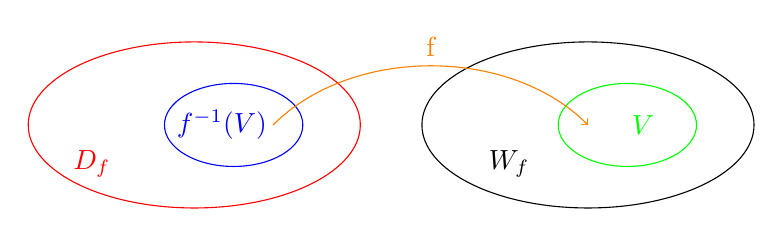
\begin{tikzpicture} 
		\draw[color=black] (5,0) ellipse (60pt and 30pt); 
		\draw[color=red] (0,0) ellipse (60pt and 30pt);
		\draw[color=blue] (0.5,0) ellipse (25pt and 15pt);
		\draw[color=green] (5.5,0) ellipse (25pt and 15pt);
		
		\draw[color=black] (4,-.5) node { $\mathbb{W}_f$};
		\draw[color=red] (-1.3,-.5) node { $\mathbb{D}_f$};
		\draw[color=blue] (0.35,0) node { $f^{-1}(\mathbb{V})$};
		\draw[color=green] (5.7,0) node { $\mathbb{V}$};
		
		\draw[->,orange] (1, 0) .. controls(2, 1) and(4,1) .. node[above,sloped] {f}(5, 0);
	\end{tikzpicture}
	
\end{center}
Beispiel:\\
$f_2 :\mathbb{R}\longmapsto[0,\infty[$ mit $x\longmapsto x^2$\\

\textbullet\;\; Bestimme das Urbild von: $f_2^{-1}([0,\infty[)$



\begin{center}
	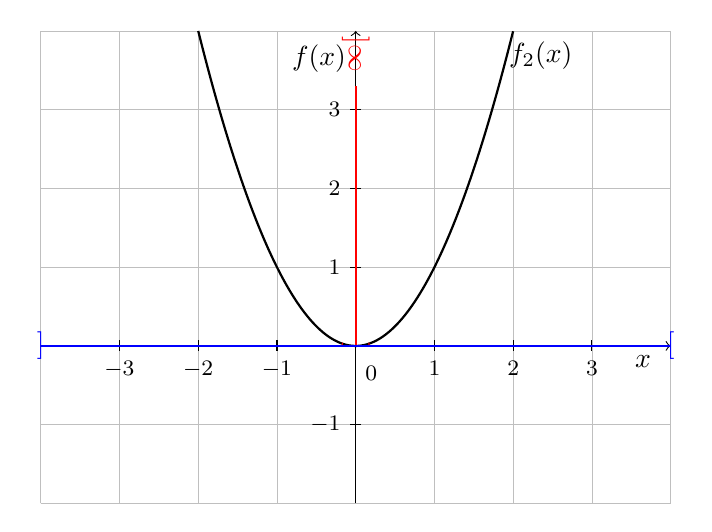
\begin{tikzpicture}
		
		% Gitternetzlinien
		\draw[xstep=1cm, ystep=1cm, very thin, color=lightgray] (-4,4) grid (4,-2);
		% x-Achse
		\draw[->] (-4,0) -- (4,0) node[below,xshift=-1em] {$x$}; 
		%Zahlen auf x-Achse
		\foreach \x in {-3,...,-1}
		\draw[shift={(\x,0)},color=black] (0pt,2pt) -- (0pt,-2pt) node[below] {\footnotesize $\x$};
		\foreach \x in {1,...,3}
		\draw[shift={(\x,0)},color=black] (0pt,2pt) -- (0pt,-2pt) node[below] {\footnotesize $\x$};
		% y-Achse 
		\draw[->] (0,-2) -- (0,4) node[left,yshift=-1em] {$f(x)$};%node[above left]
		%Zahlen auf y-Achse
		\foreach \y in {-1,...,-1}
		\draw[shift={(0,\y)},color=black] (2pt,0pt) -- (-2pt,0pt) node[left] {\footnotesize $\y$};
		\foreach \y in {1,...,3}
		\draw[shift={(0,\y)},color=black] (2pt,0pt) -- (-2pt,0pt) node[left] {\footnotesize $\y$};
		%Ursprung
		\draw[color=black] (0pt,-10pt) node[right] {\footnotesize $0$};
		
		
		
		\draw[thick,color=black] plot[samples=200, domain=-2:2] 
		(\x,{\x*\x}) node[below, xshift=1em]{$f_2(x)$};
		\draw[thick,color=red] (0,3.7) node[rotate=-90] {$]\infty$};
		\draw[thick,color=red] (0,0) node[rotate=-90] {$]$};
		\draw[thick,color=red] (0,0) -- (0,3.3); 
		\draw[color=blue,thick] (-4,0) -- (4,0) node {$[$};
		\draw[color=blue,thick] (-4,0) node {$]$}; 
	\end{tikzpicture}\\
	
\end{center}
\begin{align*}
	f_2^{-1}(\textcolor{red}{[0,\infty[})=\textcolor{blue}{\mathbb{R}}
\end{align*}

\textbullet\;\; Bestimme das Urbild von: $f_2^{-1}([2,4])$
\begin{center}
	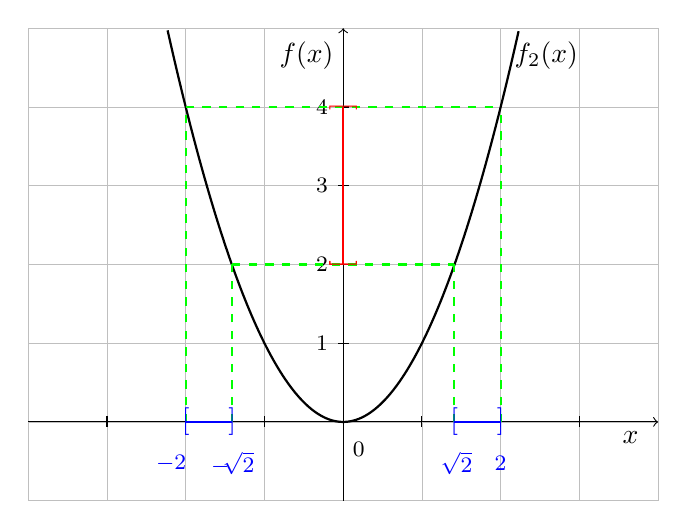
\begin{tikzpicture}
		
		% Gitternetzlinien
		\draw[xstep=1cm, ystep=1cm, very thin, color=lightgray] (-4,5) grid (4,-1);
		% x-Achse
		\draw[->] (-4,0) -- (4,0) node[below,xshift=-1em] {$x$}; 
		%Zahlen auf x-Achse
		\foreach \x in {-3,...,-1}
		\draw[shift={(\x,0)},color=black] (0pt,2pt) -- (0pt,-2pt);
		\foreach \x in {1,...,3}
		\draw[shift={(\x,0)},color=black] (0pt,2pt) -- (0pt,-2pt);
		\draw[color=blue] (-1.8,-15pt) node[right] {\footnotesize $- \sqrt[]{2}$};
		\draw[color=blue] (-2.5,-15pt) node[right] {\footnotesize $-2$};
		\draw[color=blue] (1.2,-15pt) node[right] {\footnotesize $ \sqrt[]{2}$};
		\draw[color=blue] (1.8,-15pt) node[right] {\footnotesize $2$};
		% y-Achse 
		\draw[->] (0,-1) -- (0,5) node[left,yshift=-1em] {$f(x)$};%node[above left]
		%Zahlen auf y-Achse
		%\foreach \y in {0,...,-1}
		%\draw[shift={(0,\y)},color=black] (2pt,0pt) -- (-2pt,0pt) node[left] {\footnotesize $\y$};
		\foreach \y in {1,...,4}
		\draw[shift={(0,\y)},color=black] (2pt,0pt) -- (-2pt,0pt) node[left] {\footnotesize $\y$};
		%Ursprung
		\draw[color=black] (0pt,-10pt) node[right] {\footnotesize $0$};
		
		
		
		\draw[thick,color=black] plot[samples=200, domain=-2.23:2.23] 
		(\x,{\x*\x}) node[below, xshift=1em]{$f_2(x)$};
		\draw[color=green,dashed,thick] (-2,4) -- (2,4);
		\draw[color=green,dashed,thick] (-2,0) -- (-2,4);
		\draw[color=green,dashed,thick] (2,0) -- (2,4);
		\draw[color=red,thick] (0,2)node[rotate=90] {[} -- (0,4);
		\draw[color=green,dashed,thick] (-1.41,2) -- (1.41,2);
		\draw[color=green,dashed,thick] (-1.41,0) -- (-1.41,2);
		\draw[color=green,dashed,thick] (1.41,0) -- (1.41,2);
		\draw[color=blue,thick] (-2,0)node{[} -- (-1.41,0)node{]};
		\draw[color=blue,thick] (1.41,0)node{[} -- (2,0)node{]};
		\draw[color=red,thick] (0,2)node[rotate=90] {[} -- (0,4)node[rotate=90] {]};
		
	\end{tikzpicture}\\
\end{center}
\begin{align*}
	f_2^{-1}(\textcolor{red}{[2,4]})=\textcolor{blue}{[-2,-\sqrt{2}]\cup[\sqrt{2},2]}
\end{align*}
\textbullet\;\; Bestimme das Urbild von: $f_2^{-1}(\{9\})$
\begin{center}
	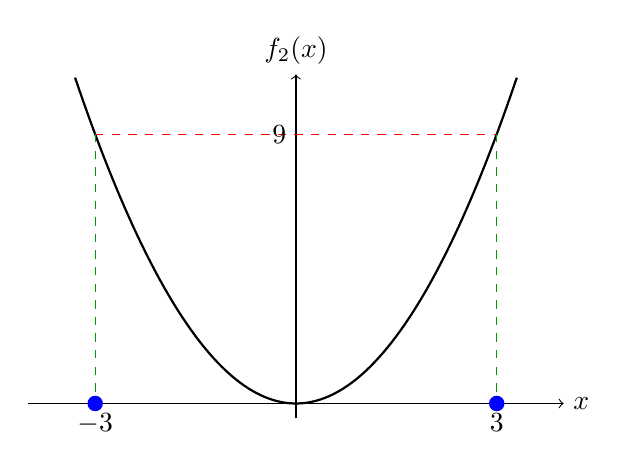
\begin{tikzpicture}[x=0.85cm,y=0.38cm]
\draw[->] (-4,0)--(4,0) node[right] {$x$};
\draw[->] (0,-0.5)--(0,11) node[above] {$f_2(x)$};
\draw[thick,domain=-3.3:3.3,samples=100] plot (\x,{\x*\x});
\draw[red,dashed] (-3,9)--(3,9);
\draw[green!60!black,dashed] (-3,9)--(-3,0) (3,9)--(3,0);
\fill[blue] (-3,0) circle[radius=2.8pt] (3,0) circle[radius=2.8pt];
\node[below] at (-3,0) {$-3$};
\node[below] at (3,0) {$3$};
\node[left] at (0,9) {$9$};
\end{tikzpicture}\\
\end{center}
\begin{align*}
	f_2^{-1}(\textcolor{red}{\{9\}})=\textcolor{blue}{\{-3,3\}}
\end{align*}
\subsection{Aufgabe zum Thema Bild und Urbild}

Sei $f:\mathbb{R}\longmapsto \mathbb{R}$ mit $f(x)=2x^2-2$ gegeben.\vspace*{2mm}\\
\begin{tabular}[t]{lll}% l=linksbündig r=rechtsbündig
	(i) & Bestimme $\mathrm{Bild}(f)$.  \\
	(ii) & Berechne $f^{-1}([6,30])$. \\
	(iii)&Berechne $f^{-1}(\{\frac{23}{7}\})$.\\	
\end{tabular} \vspace*{2mm}\\
zu (i):
\begin{quote}
	$\mathrm{Bild}(f)=?$\\
	Im positiven Bereich, wenn man große x-Werte in $f(x)$ einsetzt laufen die Werte in das Unendliche $\Rightarrow\infty [ $ .\\
	Die Funktion kann nicht kleiner als -2 werden $\Rightarrow [-2$ .\\
	\begin{align*}
		\mathrm{Bild}(f)=[-2,\infty[
	\end{align*}
\end{quote}
\begin{center}
	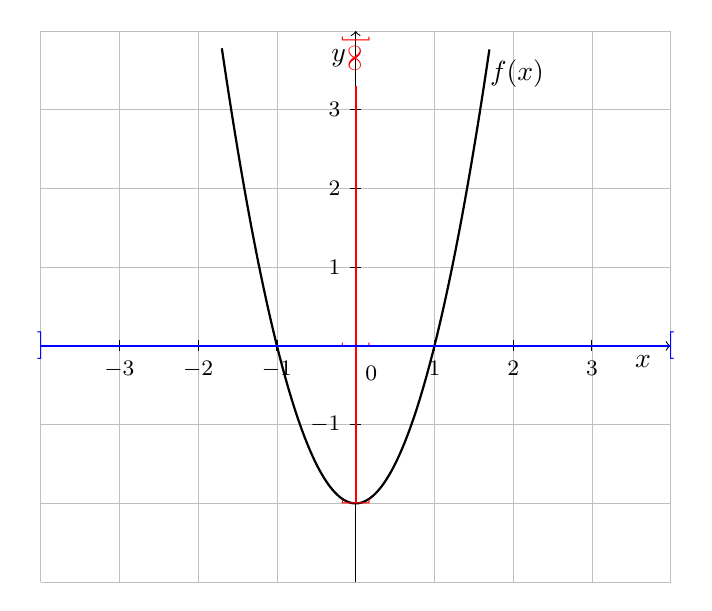
\begin{tikzpicture}
		
		% Gitternetzlinien
		\draw[xstep=1cm, ystep=1cm, very thin, color=lightgray] (-4,4) grid (4,-3);
		% x-Achse
		\draw[->] (-4,0) -- (4,0) node[below,xshift=-1em] {$x$}; 
		%Zahlen auf x-Achse
		\foreach \x in {-3,...,-1}
		\draw[shift={(\x,0)},color=black] (0pt,2pt) -- (0pt,-2pt) node[below] {\footnotesize $\x$};
		\foreach \x in {1,...,3}
		\draw[shift={(\x,0)},color=black] (0pt,2pt) -- (0pt,-2pt) node[below] {\footnotesize $\x$};
		% y-Achse 
		\draw[->] (0,-3) -- (0,4) node[left,yshift=-1em] {$y$};%node[above left]
		%Zahlen auf y-Achse
		\foreach \y in {-1,...,-1}
		\draw[shift={(0,\y)},color=black] (2pt,0pt) -- (-2pt,0pt) node[left] {\footnotesize $\y$};
		\foreach \y in {1,...,3}
		\draw[shift={(0,\y)},color=black] (2pt,0pt) -- (-2pt,0pt) node[left] {\footnotesize $\y$};
		%Ursprung
		\draw[color=black] (0pt,-10pt) node[right] {\footnotesize $0$};
		
		
		
		\draw[thick,color=black] plot[samples=200, domain=-1.7:1.7] 
		(\x,{2*\x*\x-2}) node[below, xshift=1em]{$f(x)$};
		\draw[thick,color=red] (0,3.7) node[rotate=-90] {$]\infty$};
		\draw[thick,color=red] (0,0) node[rotate=-90] {$]$};
		\draw[thick,color=red] (0,-2) node[rotate=-90] {$]$}-- (0,3.3); 
		\draw[color=blue,thick] (-4,0) -- (4,0) node {$[$};
		\draw[color=blue,thick] (-4,0) node {$]$}; 
	\end{tikzpicture}\\
	
	
\end{center}
zu (ii):
\begin{quote}
	Bestimme Urbild von: $f^{-1}({[6,30]})$\vspace*{2mm}\\
	Berechnung der Intervallgrenzen:\\
	$\blacktriangleright \quad f(x)=6\Leftrightarrow 2x^2-2=6\Leftrightarrow 2x^2=8\Leftrightarrow x^2=4 \Rightarrow x_{1,2}=\pm 2 $\\
	$\blacktriangleright \quad f(x)=30\Leftrightarrow2x^2-2=30\Leftrightarrow x^2=16\Rightarrow x_{1,2}=\pm 4$\\
	\begin{align*}
		f^{-1}([6,30])=[-4,-2]\cup [2,4]
	\end{align*}
\end{quote}
\begin{center}
	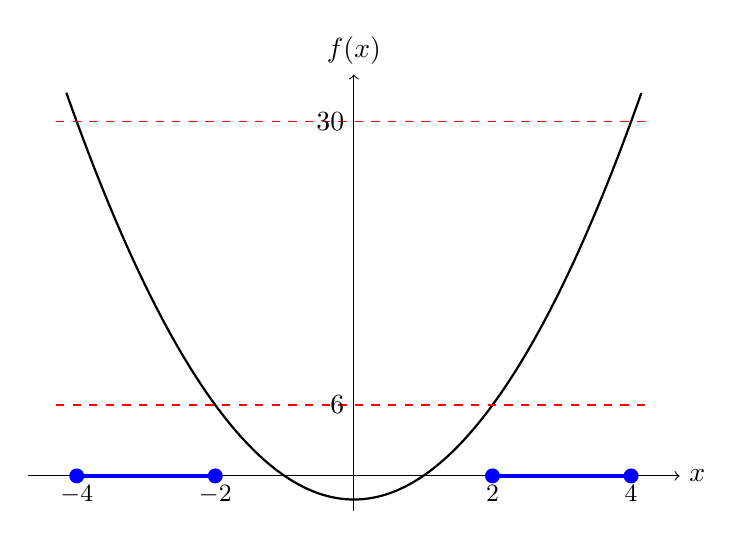
\begin{tikzpicture}[x=0.88cm,y=0.15cm]
\draw[->] (-4.7,0)--(4.7,0) node[right] {$x$};
\draw[->] (0,-3)--(0,34) node[above] {$f(x)$};
\draw[thick,domain=-4.15:4.15,samples=120]
  plot (\x,{2*\x*\x-2});
\draw[red,dashed] (-4.3,6)--(4.3,6);
\draw[red,dashed] (-4.3,30)--(4.3,30);
\node[left] at (0,6) {$6$};
\node[left] at (0,30) {$30$};
\draw[blue,ultra thick] (-4,0)--(-2,0) (2,0)--(4,0);
\foreach \x in {-4,-2,2,4}{
 \fill[blue] (\x,0) circle[radius=2.7pt];
 \node[below] at (\x,0) {\small $\x$};
}
\end{tikzpicture}\\
\end{center}
zu (iii):\\
\begin{quote}
	Bestimme Urbild von: $f^{-1}(\{\frac{23}{7}\})$\vspace*{2mm}\\
	Berechnung des Urbildes:\\
	$\blacktriangleright\quad f(x)=\frac{23}{7}	\Leftrightarrow 2x^2-2=\frac{23}{7}\Leftrightarrow 2x^2=\frac{23}{7}+2=\frac{37}{7}\Leftrightarrow x^2=\frac{37}{14}\Rightarrow x_{1,2}=\pm \sqrt{\smash[b]{\scriptscriptstyle\frac{37}{14}}}$\\
	\begin{align*}
		f^{-1}(\{\tfrac{23}{7}\})=\{ -\sqrt{\scriptscriptstyle\frac{37}{14}},\sqrt{\scriptscriptstyle\frac{37}{14}}\}
	\end{align*}
\end{quote}
\begin{center}
	\begin{tikzpicture}[x=1.3cm,y=0.75cm]
\draw[->] (-2.4,0)--(2.4,0) node[right] {$x$};
\draw[->] (0,-2.5)--(0,6) node[above] {$f(x)$};
\draw[thick,domain=-2:2,samples=120]
  plot (\x,{2*\x*\x-2});
\draw[red,dashed] (-2,3.285714)--(2,3.285714);
\node[left] at (0,3.285714) {$\frac{23}{7}$};
\draw[green!60!black,dashed]
  (-1.625687,3.285714)--(-1.625687,0)
  (1.625687,3.285714)--(1.625687,0);
\fill[blue] (-1.625687,0) circle[radius=2.5pt];
\fill[blue] (1.625687,0) circle[radius=2.5pt];
\node[below,align=center] at (-1.625687,0)
  {\scriptsize $-\sqrt{\frac{37}{14}}$};
\node[below,align=center] at (1.625687,0)
  {\scriptsize $\sqrt{\frac{37}{14}}$};
\end{tikzpicture}\\
\end{center}